\chapter{Exhaustive pseudonoise search}
  \section{Previous work}

  As shown in the previous chapter, arithmetic methods for finding sequences
  with a low off-peak autocorrelation have huge constraints on the length of
  the generated sequences. To overcome this limitation, exhaustive searches
  through the possible permutations have been conducted in the past. This
  exhaustive searchs have, if not properly optimized, a search space of
  $O(2^n)$, where $n$ is the length of the binary sequence, which make their
  results very limited by computational complexity.\\

  Some developments have been conducted in the past for aperiodic
  autocorrelation optimization. Even though we are searching for periodic
  autocorrelation rather than aperiodic ones, these works are worth looking
  at them:\\

  First of all, we are going to take a look at the definition of the
  aperiodic autocorrelation:\\
  \begin{definition}[Aperiodic autocorrelation]
      Given a binary sequence $S$, we define its aperiodic autocorrelation as:
      \begin{equation}
        A'_{\tau}(S) = \sum_{i=1}^{N-\tau}s_{i}s_{i+\tau}
      \end{equation}
  \end{definition}

  All these works focus on finding a sequence $S$ that minimizes:

  \begin{definition} Given a binary sequence $S$, we define the energy of $S$
    as:
    \begin{equation}
      E(S) = \sum_{i=1}^{N-1} A'^{2}_{k}(S)
    \end{equation}
    \begin{equation}
      E_{min} = \operatorname*{min}_{subset} \sum_{i=1}^{N-1} A'^{2}_{k}
    \end{equation}
  \end{definition}

  One of the first optimizations for this method was
  proposed by \citet{Mertens_1996} in which he provided an algorythm
  with a complexity of $O(1.85^n)$. In his work, he applied a branch and bound
  algorythm that rules out the equivalent sequences and sets a minimum bound
  to the autocorrelation based on how complementing a single symbol of the
  sequence affects the autocorrelation.\\

  First of all, the recursion is done by picking a sequence and recursivily
  fixing elements at the extremes of the sequence as shown in Figure
  \ref{prn_search:fig:1}.\\

  \begin{figure}[ht!]
    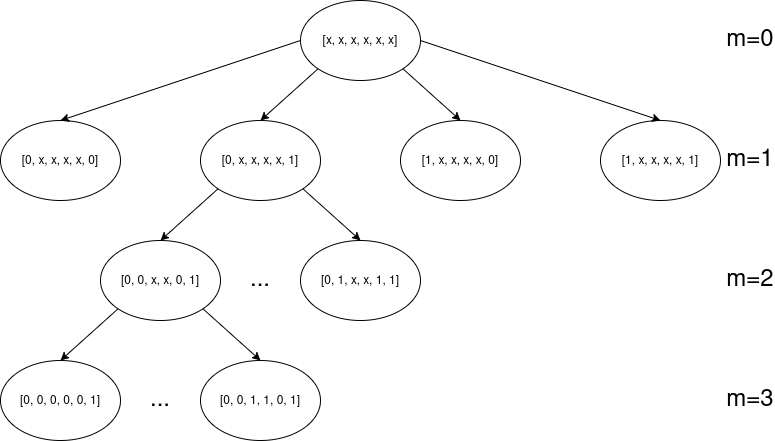
\includegraphics[scale=0.6]{Chapters/prn_search/branching_example.png}
    \caption{An example of the branching used in \citet{Mertens_1996} with
    $N = 6$ and where x represent unfixed values.}
    \label{prn_search:fig:1}
  \end{figure}

  It's trivial that, when we complement a sequence, the components of the
  autocorrelation can be lowered by, at most, -2. Based on that, we can get a
  relaxation of $E_{min}$:\\
  \begin{equation}
    E_b = \sum_{k=1}^{N-1}max\{b_k, (|A'_k| - 2f_k)^2\} \leq E_{min}
  \end{equation}
  where $A'_k$ is the autocorrelation of an arbitrary sequence, $b_k = (N -
  k) \bmod 2$ the minimum possible value for $|A'_k|$ and $f_k$ the number of
  unfixed elements in $A'_k$ given by:
  \begin{equation}
    f_k = \left\{\begin{array}{ll}
        0 & k \geq N - m \\
        2(N - m - k) & N/2 \leq k < N - m\\
        N - 2m & k < N/2 \\
    \end{array}\right.
  \end{equation}

  where $N$ is the size of the sequence to search and $m$ the number of fixed
  elements at the extremes of the sequence.\\

  If $E_b$ is greater than the best candidate for $E_{min}$ so far, we can
  prune that branch reducing the amount of computation. With this algorythm,
  Mertens optimized sucessfully up to $N = 48$.\\

  This work was further improved in \citet{Packebusch_2016}. In this paper,
  they review 2 bounds provided by different authors(Prestwich and
  Wiggenbrock) and combine them to create a new bound that lowers the
  complexity to $O(1.729^N)$, solving the LABS problem up to $N = 66$. This
  record was broken by \citet{anatoli} by computing it up to $N = 85$.\\

  \section{Our approach}

  To tackle the huge complexity encountered in the previous methods, a different
  approach was taken. Instead of dealing with the combinatorial explosion
  of all the possible binary sequences of length $N$, we decided to work with
  a smaller set consisting on all the possible sequences which can be
  constructed through the composition method with Legendre base sequences.\\

  This approach haves some pros and cons. First of all, the search space is
  reduced from $O(2^N)$ to $O(p^m)$ where $p*m = N$. This clearly means that
  the complexity grows much more smoothly than in previous works. In fact, the
  autocorrelation function can be optimized for sequences generated through the
  composition method as shown in a following chapter.\\

  The problem is that the possible sizes for the sequences are limited as $n$
  and $p$ are required to fulfill $gcd(p, m) = 1$. Even though it means that
  these method cannot find optimal sequences for all lengths, the restriction is
  looser than the non-exhaustive methods. Apart from that, this method doesn't
  explore all possible permutations and it doesn't ensure to find a pseudonoise
  sequence if it exists. To sum up, this method has been proven useful
  through examples as a good way to construct useful sequences but shouldn't
  be used to prove the non existence of pseudonoise sequences for a given
  length.\\

  Given a base sequence of size $n$ and a length $m$ for the shift sequences,
  our program needs to find all the shift sequences that generate a composite
  sequence with a good autocorrelation.\\

  This means that the search space are all the posible permutations of the
  shift sequence, in other words, $n^m$ permutations. However, there are some
  relations between the different shift sequences that let us narrow the
  search space.\\

  For example, if we add a constant to every component to the shift sequence,
  we get a shifted version of the same sequence. This means that if we only
  computed the permutations that start with the same component, we would cover
  the whole search space as any other permutations would just be shifts of
  one permutation from the computed set. This optimization narrows our
  search space to $n^{(m-1)}$.\\

  Other optimization arises from the form of the shift sequences. In general,
  if the symbols are repeated often, they trend to generate higher
  autocorrelation spikes or periods inside the composite sequence. This
  concept can be easily expressed with the Hamming autocorrelation function:\\

  \begin{definition}[Hamming autocorrelation]
    Given a sequence $S$ of length $n$ and the function $shift$ defined at
    Equation \ref{eq:3}, we define the Hamming autocorrelation as:
      \begin{equation} \label{hamming:eq:1}
        HA(S)_{\tau} = \sum_{i=1}^{n} HAComponent(S_{\tau}, shift(S, \tau)_{\tau})
      \end{equation}
    where $HAComponent$ is defined as:
      \begin{equation}
        HAComponent(c1, c2) = \left\{\begin{array}{lr}
            1  &  c1 = c2\\
            0  & \textnormal{otherwise} \\
        \end{array}\right.
      \end{equation}
  \end{definition}

  For our branch and bound algorythm, it's important to note that if we
  substitute a symbol that only appears once for another, the hamming
  autocorrelation won't get lower. This means that if we do a depth-in-first
  bounding the nodes that have a hamming autocorrelation higher than the
  threshold (we mean, the maximum non trivial component), we are sure that all
  nodes in that branch have a higher hamming autocorrelation than the
  threshold. This means that when the threshold is supassed, the branch can
  be safely prune and save a lot of computation time.\\

  \begin{figure}[ht!]
    \begin{center}
      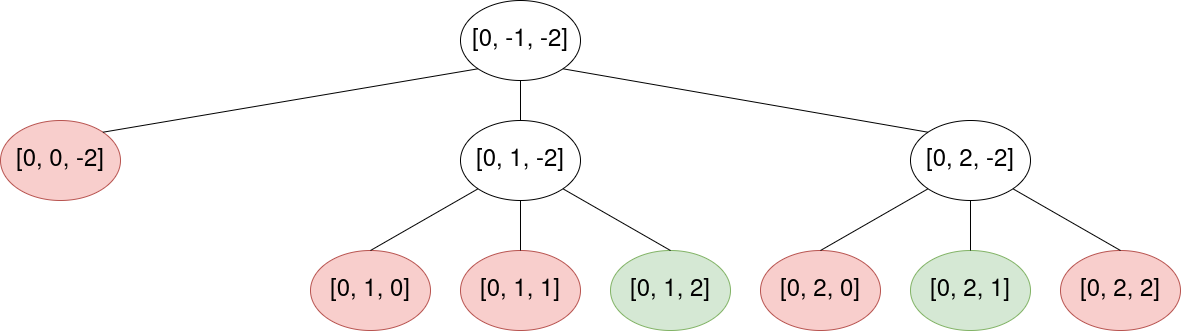
\includegraphics[scale=0.4]{Chapters/Implementation/Example_branch_bound.png}
    \end{center}
    \caption{An example of the branch and bound algorythm with a threshold for
    hamming autocorrelation of 1 and a base sequence of length 3. Red nodes
    represent prunes and green ones final nodes in which the
    autocorrelation is computed and checked. Negative values represent those
    that haven't been initialized yet.}
    \label{bb:fig:1}
  \end{figure}

  We can deduce several things from Figure \ref{bb:fig:1}:
  \begin{itemize}
    \item We reduce the number of autocorrelations computed by a significant
    amount.
    \item The computation on each branch isn't balanced. This must be taken
    into account when we design the parallelism model.
  \end{itemize}
